\section{Tahap Perancangan Kapal}
\label{sec:tahap-deskap}

\begin{figure}[!ht]
    \centering
    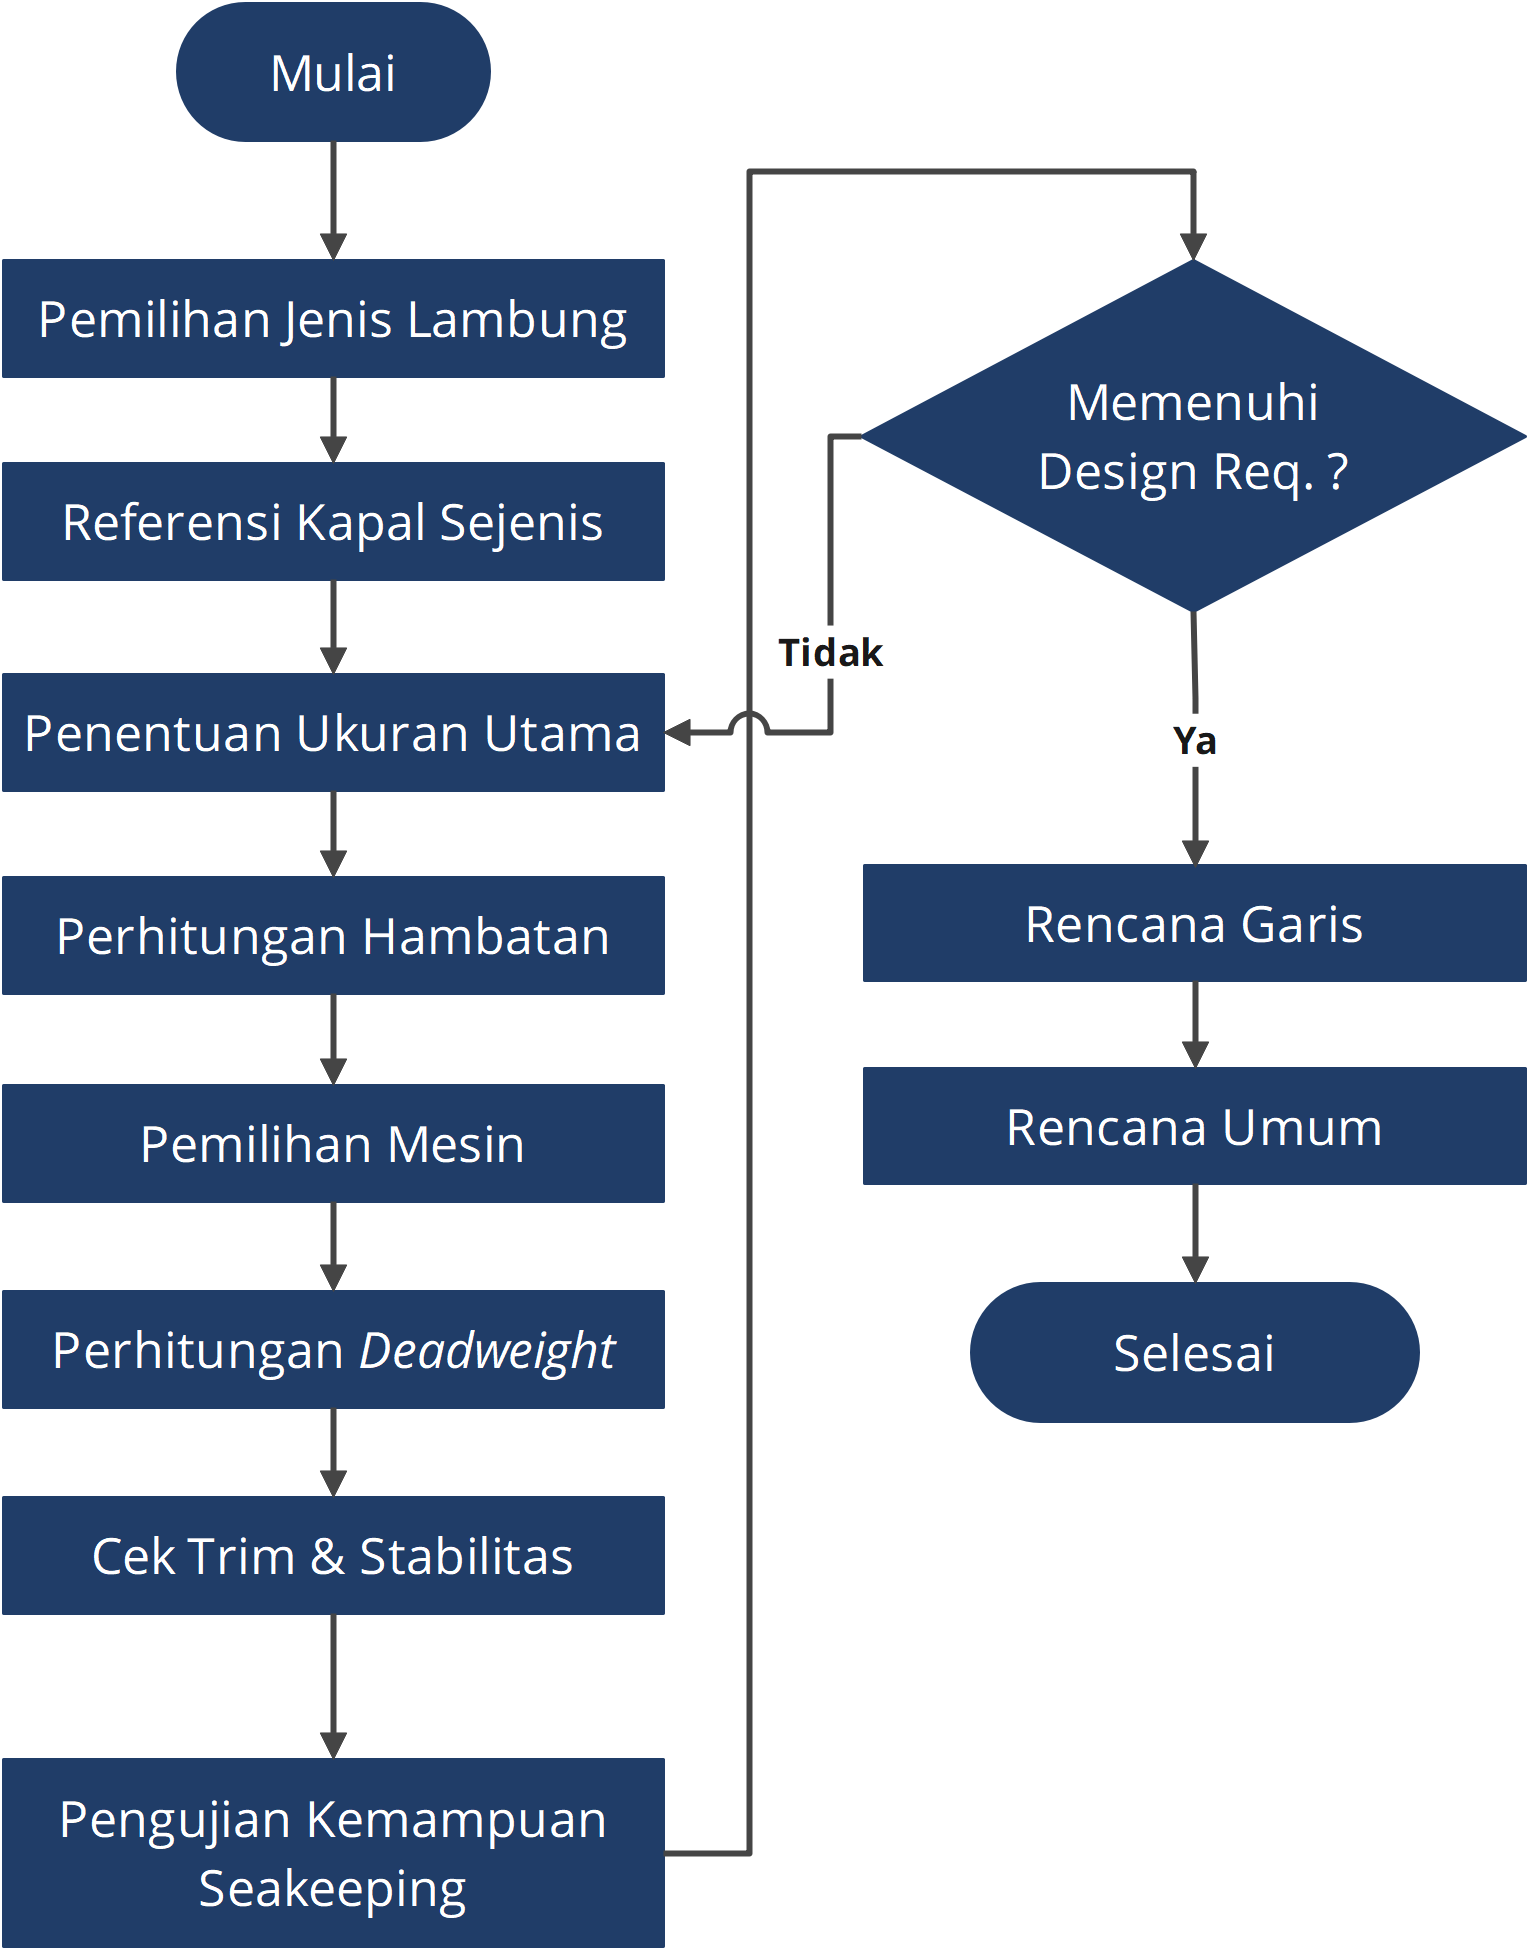
\includegraphics[width=0.42\textwidth]{gambar/FC_Deskap.png}
    \caption{Diagram Alir Perancangan Kapal}
    \label{fig:flowchart-deskap}
\end{figure}

Luaran tahap berikutnya merupakan spesifikasi kapal yang akan di desain. Proses pertama yang dilakukan adalah merencanakan bentuk lambung kapal melalui pembuatan rencana garis. Perencanaan bentuk lambung ini dilakukan dengan bantuan perangkat lunak \emph{Maxsurf Modeler}. Faktor yang-yang harus diperhatikan adalah \emph{Displacement} dan ukuran-ukuran utama yang telah dihitung sebelumnya tetap sesuai dengan bentuk lambung kapal yang dirancang.

Setelah rencana garis selesai, ruangan-ruangan yang ada di kapal dirancang agar sesuai dengan perhitungan dan dilakukan koreksi-koreksi agar desain kapal sesuai. Volume muatan yang dibawa, jumlah akomodasi yang dibutuhkan, ukuran ruang mesin dan kaidah konstruksi kapal menjadi patokan utama dalam penentuan dan penataan ruangan yang ada di kapal.

Kriteria \emph{sea keeping} dan stabilitas akan menjadi sorotan utama dalam penelitian ini. Kapal yang dirancang harus mampu beroperasi didalam kondisi lingkungan sesuai dengan pola operasi yang direncanakan berdasarkan hasil simulasi dan optimasi. Hal ini dikarenakan cakupan penelitian ini adalah aapakah bisa mengatasi masalah kelangkaan BBM yang ada dengan cara mengganti moda pemasokan.

Koreksi dilakukan dalam penentuan volume tangki yang ada, hal ini karena peletakan batasan antar tangki harus diletakkan di gading besar. Koreksi berikutnya menentukan letak tangki-tangki bagian \emph{consumables} agar trim kapal memenuhi peraturan yang berlaku.

Setelah penataan ruangan hal yang harus direncakan berikutnya adalah peralatan keselamatan yang harus dimiliki oleh kapal yang dirancang. Jumlah kru kapal, muatan yang dibawa, ukuran kapal dan regulasi SOLAS menjadi hal yang mempengaruhi peralatan dan perlengkapan apa yang harus dibawa oleh kapal.
